\chapter{Desenvolvimento}
\label{desenvolvimento}
Desenvolvimento sob a perspectiva da Interação Humano-Computador. "Organização do Espaço de Problema e Análise de Tarefas" que aborda a importância de compreender as características dos usuários e seu relacionamento com a tecnologia. Destaca-se a necessidade de agrupar os usuários por características semelhantes para desenvolver interfaces adequadas às suas necessidades. Em seguida, são apresentadas as subseções: "Perfil de usuário", que descreve as características dos usuários-alvo do projeto; "Personas", que apresenta duas personas específicas com seus objetivos e interesses; "Cenários - Análise de cenário de problema", que descreve a aplicação do jogo What Weee Are em uma sala de aula e a experiência de duas pessoas jogando; e "Análise Hierárquica de Tarefas", que inclui figuras com a análise detalhada das tarefas envolvidas no jogo.

\section{Organização do Espaço de Problema e Análise de Tarefas}
A organização do espaço de trabalho é fundamental para garantir uma interação humano-computador (IHC) eficaz e eficiente. Para isso, é preciso levar em consideração uma série de fatores, como a descrição detalhada das características dos usuários, suas necessidades, habilidades e limitações, sua relação com a tecnologia e o ambiente em que irão utilizar o sistema. No contexto da IHC, é importante compreender o perfil dos usuários que irão interagir com o sistema, incluindo informações como idade, nível de escolaridade, habilidades técnicas, experiência com tecnologia e com o tema específico do sistema em questão. Essas informações podem ser obtidas por meio de pesquisas de campo, entrevistas e estudos de usabilidade. Ao agrupar os usuários por características semelhantes, é possível ambientar melhor o projeto, com interfaces e funcionalidades que atendam às necessidades específicas de cada grupo de usuários. Por exemplo, no presente trabalho, o foco está em pessoas de idade escolar, com interesse em tecnologia e baixa experiência ou contato com assuntos ambientais. Nesse caso, a organização do espaço de trabalho deve levar em consideração essas características e desenvolver interfaces intuitivas e amigáveis, com informações e funcionalidades relevantes para esse público específico.

Alessio desempenhou um papel central na co-criação do projeto What Weee Are, atuando como principal idealizador e contribuindo significativamente para a concepção e desenvolvimento do jogo. As interações iniciais ocorreram por meio de duas reuniões realizadas via Google Meet, nas quais Alessio compartilhou suas ideias iniciais e contribuiu para a elaboração da estrutura do jogo, incluindo a ideia de desmontar itens durante o jogo, a obtenção de poderes e a criação de quatro fases distintas.

Além disso, Alessio contribuiu fornecendo arte para ser utilizada no jogo e participou ativamente das decisões relacionadas às fases, que foram definidas como cozinha, jardim, metrô e vulcão. Sua origem italiana foi fundamental para a tradução do jogo para o idioma, e ele também ofereceu sugestões valiosas para a implementação de detalhes importantes no jogo. Como resultado de sua colaboração, o jogo What Weee Are se tornou um produto mais completo e diversificado, com uma abrangência maior e a possibilidade de atender a um público internacional.

\subsection{Perfil de usuário}
Sob a óptica de IHC, se trata da descrição detalhada das características dos usuários, sua relação com tecnologia, seu conhecimento sobre domínio e tarefas, agrupar usuários por características semelhantes. Neste trabalho, o foco são em pessoas de idade escolar majoritariamente, mas não excludente à pessoas fora desta faixa. Com interesse por tecnologias e com baixa experiência ou contato pelo assunto ambiental. Olhar tabela \ref{table:personasTable}
\begin{table}[h]
    \centering
    \begin{tabular}{|l|l|l|}
        \hline
                                 & Aluno A     & Aluno B      \\ \hline
        Faixa etária             & 5 a 12 anos & 13 a 17 anos \\ \hline
        Interesse por tecnologia & sim         & sim          \\ \hline
        Experiência ambiental    & baixa       & baixa        \\ \hline
    \end{tabular}
\caption{Tabela de personas}
\label{table:personasTable}
\end{table}

\subsection{Personas}
João Pedro é um professor da Escola Estadual João Carlos Gomes Cardim, em Diadema, hoje leciona para o quinto ano do ensino fundamental. Gosta de trazer aulas dinâmicas aos alunos, pois entende que isso os prende com maior atenção ao que está sendo lecionado. Entende que o uso da tecnologia no ensino pode ser uma ferramenta muito auxiliadora, uma vez que, os alunos gostam de ficar conectados e praticamente passaram a vida toda em contato com o mundo digital.
Têm como objetivos pessoais promover uma educação ativa com os alunos, colocar em evidência os Objetivos de Desenvolvimento Sustentável para os alunos.
Objetivos Pessoais: 
- Aprimorar o aprendizado de seus alunos sobre os problemas causados pelo desperdício de materiais eletrônicos.

Objetivos Práticos:
- Levar um jogo divertido sobre o assunto aos seus alunos;
- Engajar os alunos sobre assuntos que normalmente são ignorados.


Natália é aluna do sexto ano do ensino fundamental e aluna do professor João Pedro. Gosta de videogames, assim como outras crianças de sua idade, possui um interesse grande em tecnologia e pelo mundo digital.

Leonardo é aluno do primeiro ano do ensino médio, da Escola Estadual João Carlos Gomes Cardim, em Diadema. Possui interesse em cursar faculdade de biologia na UFABC, pois após uma visita a instituição chegou a informação da interdisciplinaridade e vê isso como uma boa oportunidade de realizar projetos envolvendo biologia e computação, que é o seu segundo interesse.

\subsection{Cenários - Análise de cenário de problema}
\label{cenarios}
O Professor João Pedro, resolveu trazer novas maneiras de ministrar suas aulas sobre sustentabilidade, e viu uma oportunidade de fazer isso via jogos digitais, uma vez que tem conhecimento da preferência de seus alunos por tecnologia. Trouxe para a turma do sexto ano, de Natália, o jogo digital What Weee Are para abordar tais assuntos de maneira lúdica e mais ativa por partes dos alunos, uma vez que eles que irão interagir com o sistema. A ideia é requisitar uma redação sobre reciclagem de materiais eletrônicos antes e após a partida jogada pelos alunos. O Professor acredita que a apresentação do jogo aos alunos irá proporcionar dinamismo e maior interesse dos alunos ao assunto sobre desperdício de materiais eletrônicos.

Natália iniciou o jogo lendo um breve diálogo explicando quais são os problemas ali enfrentados e de quais maneiras poderá ajudar a resolver este empasse. Utilizando as teclas A e D do teclado para se movimentar (A para esquerda, D para direita), ESPAÇO para pular e J para interagir com objetos e avanço de diálogos. Inicialmente houveram dificuldades para progredir, pois não foram coletados os materiais mal descartados no jogo, que são usados para possibilitar a progressão, ao entender que era necessário a coleta dos itens a dificuldade deixou de ser um problema. Natália ficou muito animada ao perceber que seu personagem poderia ficar mais forte ao progredir no jogo.

Leonardo iniciou o jogo muito interessado pelo sistema de construção e desconstrução, imaginando muitas possibilidades de novos itens e maneiras que o personagem pudesse ficar mais fortes, tentando diversas combinações de materiais para criação de outro que seja útil para progressão, logo de cara entendeu que a coleta dos recursos pelos mapas do jogo seria crucial para a evolução do jogo. Sentiu que o jogo poderia apresentar uma maior dificuldade para que houvesse mais desafios e que houvessem novas fases no jogo.

\subsection{Análise Hierárquica de Tarefas}
\begin{figure}[h]
    \centering
    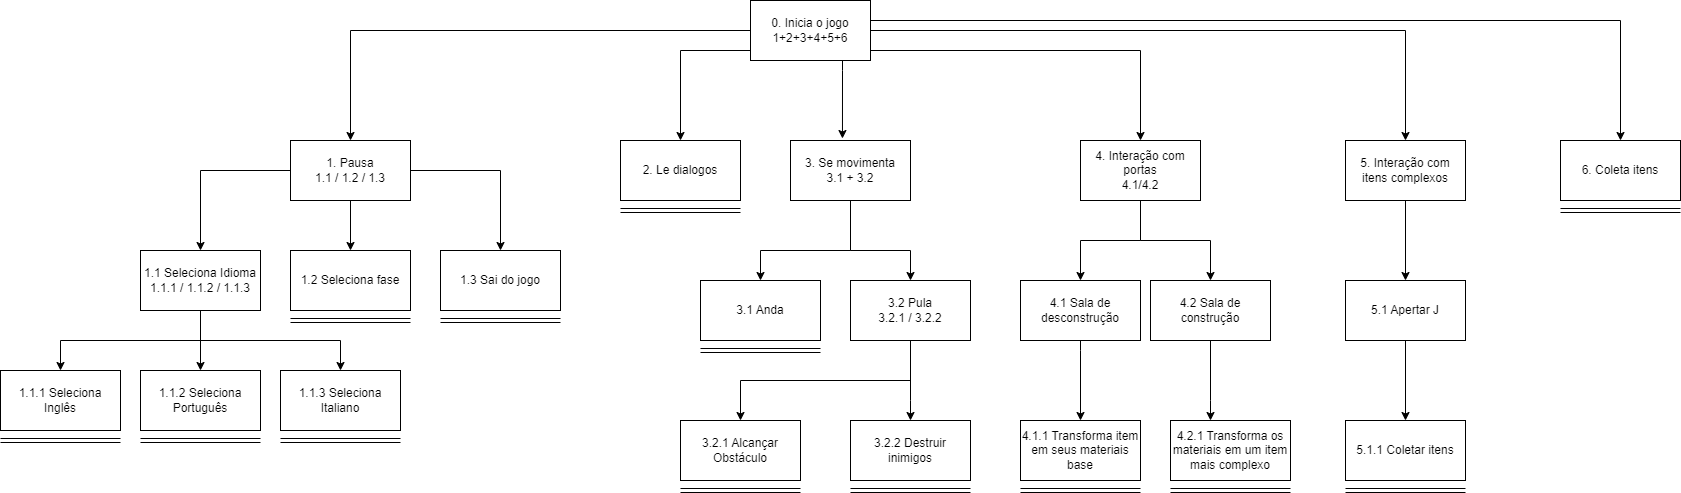
\includegraphics[width=\textwidth]{figuras/analise_tarefas.drawio.png}
    \caption{Análise Hierárquica de Tarefas}
    \label{fig_analise_hierarquica}
\end{figure}

\begin{figure}[h]
    \centering
    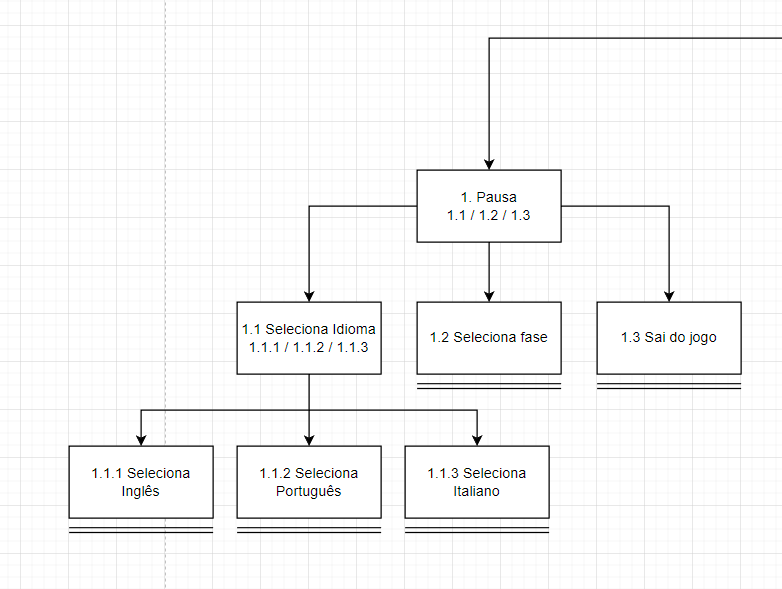
\includegraphics[width=\textwidth]{figuras/aht-a.png}
    \caption{Análise Hierárquica de Tarefas - A}
    \label{fig_analise_hierarquica_a}
\end{figure}
\begin{figure}[h]
    \centering
    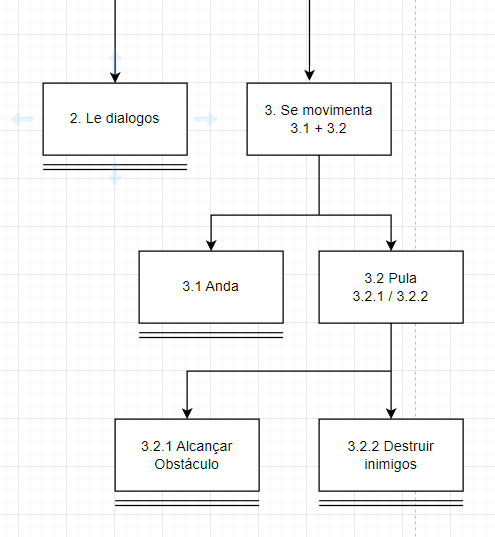
\includegraphics[width=\textwidth]{figuras/aht-b.png}
    \caption{Análise Hierárquica de Tarefas - B}
    \label{fig_analise_hierarquica_b}
\end{figure}
\begin{figure}[h]
    \centering
    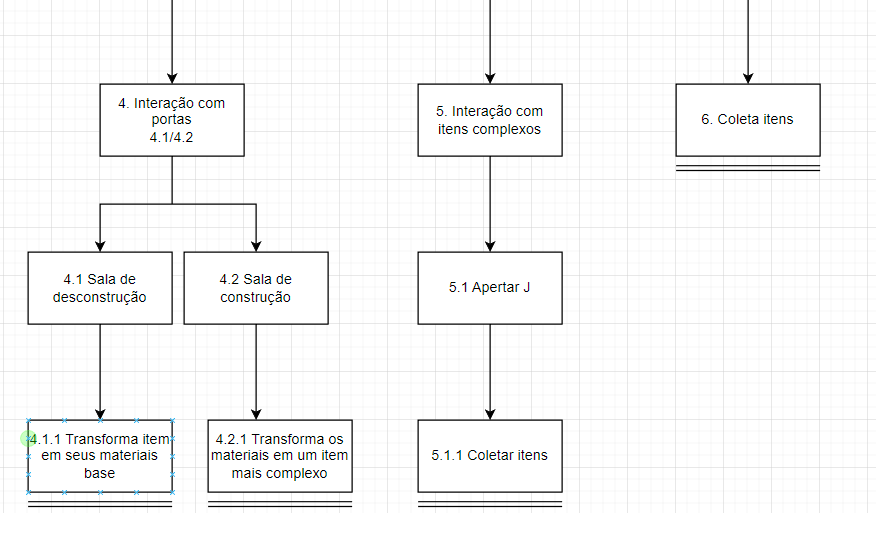
\includegraphics[width=\textwidth]{figuras/aht-c.png}
    \caption{Análise Hierárquica de Tarefas - C}
    \label{fig_analise_hierarquica_c}
\end{figure}
